% !TeX program = xelatex
\documentclass[a4paper,12pt]{article}

% ===== 1. KHỔ GIẤY, LỀ TRANG, FONT =====
\usepackage[left=3cm,right=2cm,top=2cm,bottom=2cm,footskip=1cm]{geometry}
\usepackage{fontspec}

\IfFontExistsTF{Times New Roman}{
  \setmainfont{Times New Roman}
}{
  \IfFileExists{fonts/times.ttf}{
    \setmainfont{times.ttf}[
      Path=fonts/,
      BoldFont=timesbd.ttf,
      ItalicFont=timesi.ttf,
      BoldItalicFont=timesbi.ttf]
  }{
    \IfFontExistsTF{TeX Gyre Termes}{
      \setmainfont{TeX Gyre Termes}
      \PackageWarningNoLine{MauBaoCao}{Times New Roman unavailable; using TeX Gyre Termes}
    }{
      \setmainfont{DejaVu Serif}
      \PackageWarningNoLine{MauBaoCao}{Times New Roman unavailable; using DejaVu Serif}
    }
  }
}
\usepackage{indentfirst}
\usepackage{microtype}
\usepackage{graphicx}
\usepackage{float}
\usepackage{tikz}
\usepackage{array,tabularx,booktabs,longtable}
\usepackage{enumitem}
\usepackage{titlesec}
\usepackage{tocloft}
\usepackage{caption}
\usepackage{xurl}
\usepackage[unicode,hidelinks]{hyperref}
\urlstyle{same}

\renewcommand{\normalsize}{\fontsize{13}{19.5}\selectfont}
\AtBeginDocument{\normalsize}
\setlength{\parindent}{0.5cm}
\setlength{\parskip}{4pt}
\setlength{\emergencystretch}{2em}
\raggedbottom
\setlist{topsep=4pt,itemsep=2pt,parsep=0pt,leftmargin=*}

% ===== 2. BA CẤP TIÊU ĐỀ: 1 / 1.1 / 1.1.1 =====
\setcounter{secnumdepth}{3}
\setcounter{tocdepth}{3}
\renewcommand{\thesection}{\arabic{section}}
\renewcommand{\thesubsection}{\thesection.\arabic{subsection}}
\renewcommand{\thesubsubsection}{\thesubsection.\arabic{subsubsection}}
\titleformat{\section}[hang]
  {\normalfont\fontsize{16}{20}\selectfont\bfseries}
  {\thesection.}{0.6em}{}
\titleformat{\subsection}[hang]
  {\normalfont\fontsize{14}{18}\selectfont\bfseries}
  {\thesubsection}{0.6em}{}
\titleformat{\subsubsection}[hang]
  {\normalfont\fontsize{13}{17}\selectfont\bfseries}
  {\thesubsubsection}{0.6em}{}
\titlespacing*{\section}{0pt}{16pt}{8pt}
\titlespacing*{\subsection}{0pt}{12pt}{6pt}
\titlespacing*{\subsubsection}{0pt}{8pt}{4pt}

% ===== 3. MỤC LỤC VÀ SỐ TRANG =====
\renewcommand{\contentsname}{MỤC LỤC}
\renewcommand{\refname}{Tài liệu tham khảo}
\renewcommand{\cfttoctitlefont}{\fontsize{16}{20}\selectfont\bfseries}
\setlength{\cftbeforetoctitleskip}{0pt}
\setlength{\cftaftertoctitleskip}{18pt}
\renewcommand{\cftsecfont}{\normalfont\bfseries}
\renewcommand{\cftsecpagefont}{\normalfont\bfseries}
\renewcommand{\cftsubsecfont}{\normalfont}
\renewcommand{\cftsubsubsecfont}{\normalfont}
\renewcommand{\cftsecleader}{\cftdotfill{\cftdotsep}}
\cftsetindents{section}{0em}{2em}
\cftsetindents{subsection}{2em}{3em}
\cftsetindents{subsubsection}{5em}{4em}
\setlength{\cftbeforesecskip}{6pt}
\makeatletter
\def\ps@plain{%
  \let\@oddhead\@empty\let\@evenhead\@empty
  \def\@oddfoot{\hfil{\normalfont\fontsize{11}{13}\selectfont\thepage}\hfil}%
  \let\@evenfoot\@oddfoot}
\makeatother
\pagestyle{plain}

% ===== 4. BẢNG, HÌNH, CHÚ THÍCH =====
\renewcommand{\tablename}{Bảng}
\renewcommand{\figurename}{Hình}
\DeclareCaptionFont{reportcaption}{\fontsize{12}{15}\selectfont}
\captionsetup{font=reportcaption,labelfont=bf,labelsep=period,
  justification=centering,skip=6pt}
\newcolumntype{Y}{>{\raggedright\arraybackslash}X}
\newcommand{\bangfont}{\fontsize{12}{15}\selectfont}

% ===== 5. THÔNG TIN TRANG BÌA =====
\newcommand{\DonViChuQuan}{ĐẠI HỌC QUỐC GIA HÀ NỘI}
\newcommand{\TenTruong}{TRƯỜNG ĐẠI HỌC CÔNG NGHỆ}
\newcommand{\LoaiBaoCao}{BÁO CÁO TIẾN ĐỘ DỰ ÁN 1}
\newcommand{\TenMonHoc}{ĐIỆN TOÁN ĐÁM MÂY}
\newcommand{\TenDeTai}{SatiBot -- Quản lý và tương tác với các tài nguyên AWS bằng ngôn ngữ tự nhiên}
\newcommand{\GiangVien}{TS. Hoàng Xuân Tùng}
\newcommand{\SoNhom}{Nhóm 10}
\newcommand{\LopMonHoc}{INT3319 1}
\newcommand{\DiaDiemThoiGian}{Hà Nội, Tháng 10/2026}
\hypersetup{pdftitle={BÁO CÁO TIẾN ĐỘ DỰ ÁN 1 - SATIBOT},pdfauthor={Nhóm 10}}

\begin{document}

% ===== 6. TRANG BÌA =====
\begin{titlepage}
\thispagestyle{empty}
\begin{tikzpicture}[remember picture,overlay]
  \draw[line width=2pt]
    ([xshift=3cm,yshift=-2cm]current page.north west)
    rectangle ([xshift=-2cm,yshift=2cm]current page.south east);
  \draw[line width=0.5pt]
    ([xshift=3.12cm,yshift=-2.12cm]current page.north west)
    rectangle ([xshift=-2.12cm,yshift=2.12cm]current page.south east);
\end{tikzpicture}\par
\centering
\setlength{\parindent}{0pt}
\setlength{\parskip}{0pt}
\vspace*{0.8cm}
{\fontsize{14}{18}\selectfont\bfseries\DonViChuQuan\par}
\vspace{0.15cm}
{\fontsize{15}{20}\selectfont\bfseries\TenTruong\par}
\vspace{0.25cm}
\rule{5cm}{0.4pt}\par
\vspace{0.5cm}

\IfFileExists{logo.png}{
  
\includegraphics[width=3.8cm,height=3.8cm,keepaspectratio]{logo.png}
}{
  \IfFileExists{logo_uet.png}{
    \includegraphics[width=3.8cm,height=3.8cm,keepaspectratio]{logo_uet.png}
  }{
    \fbox{\parbox[c][3.4cm][c]{3.4cm}{\centering
      \fontsize{11}{14}\selectfont LOGO TRƯỜNG}}
  }
}\par
\vspace{0.7cm}
{\fontsize{22}{27}\selectfont\bfseries\LoaiBaoCao\par}
\vspace{0.35cm}
\begin{minipage}{0.9\textwidth}\centering
  {\fontsize{15}{20}\selectfont\bfseries MÔN HỌC: \TenMonHoc\par}
\end{minipage}\par
\vspace{0.6cm}
{\fontsize{13}{17}\selectfont\bfseries ĐỀ TÀI\par}
\vspace{0.12cm}
\begin{minipage}{0.9\textwidth}\centering
  {\fontsize{16}{21}\selectfont\bfseries\TenDeTai\par}
\end{minipage}\par
\vspace{0.65cm}
{\fontsize{13}{19.5}\selectfont
\renewcommand{\arraystretch}{1.1}
\begin{tabular}{@{}>{\raggedright\arraybackslash\bfseries}p{5.2cm}>{\raggedright\arraybackslash}p{8cm}@{}}
  Giảng viên hướng dẫn: & \GiangVien\\
  Nhóm thực hiện: & \SoNhom\\
  Sinh viên thực hiện: & Cao Anh Minh \textbf{(Trưởng nhóm)}\\
                      & Trịnh Thiên Quang\\
                      & Phạm Đức Hùng\\
                      & Nguyễn Đức Huy\\
  Lớp môn học: &  \LopMonHoc
\end{tabular}\par}
\vfill
{\fontsize{13}{17}\selectfont\bfseries\DiaDiemThoiGian\par}
\vspace*{0.5cm}
\end{titlepage}

% ===== 7. MỤC LỤC TỰ ĐỘNG =====
\pagenumbering{roman}
\tableofcontents
\clearpage
\pagenumbering{arabic}

% ===== 8. NỘI DUNG BÁO CÁO =====

\section{TỔNG QUAN VỀ DỰ ÁN}

\subsection{Giới thiệu chung về tính năng dự án}

Trong bối cảnh điện toán đám mây phát triển mạnh mẽ, Amazon Web Services (AWS) đã trở thành nền tảng hạ tầng phổ biến bậc nhất hiện nay. Tuy nhiên, việc quản trị và cấu hình tài nguyên thông qua giao diện đồ họa (AWS Management Console) thường đòi hỏi người dùng phải thực hiện nhiều thao tác thủ công, điều hướng qua các bảng điều khiển phức tạp và tiềm ẩn nhiều rủi ro cấu hình sai. Ngược lại, việc sử dụng giao diện dòng lệnh (AWS CLI) hoặc các tập lệnh tự động lại đặt ra rào cản lớn về việc ghi nhớ cú pháp lệnh, định dạng tài liệu JSON cũng như quy chuẩn tham số. Đối với sinh viên, lập trình viên mới tiếp cận hạ tầng hoặc quản lý kỹ thuật, những rào cản này làm suy giảm đáng kể hiệu suất vận hành và gia tăng nguy cơ rò rỉ bảo mật hoặc phát sinh chi phí ngoài tầm kiểm soát.

Để giải quyết bài toán trên, nhóm đề xuất xây dựng SatiBot -- ứng dụng web ChatOps thông minh hỗ trợ quản trị, cấu hình và giám sát các tài nguyên đám mây AWS hoàn toàn bằng ngôn ngữ tự nhiên (được tối ưu hóa cho tiếng Việt). Bằng cách kết hợp mô hình ngôn ngữ lớn (LLM) hỗ trợ cơ chế \textit{Function Calling} cùng bộ công cụ AWS SDK (Boto3), SatiBot đóng vai trò là một trợ lý ảo DevOps trực quan. Người dùng chỉ cần gửi yêu cầu qua giao diện trò chuyện; hệ thống sẽ tự động phân tích ngữ cảnh, đối soát tính an toàn, kích hoạt các API AWS tương ứng và trả về kết quả kèm các chỉ số thống kê, liên kết bảo mật hoặc cảnh báo rủi ro một cách minh bạch và chuẩn hóa.

\subsection{Giới thiệu người dùng của dự án}

Hệ thống SatiBotBot được thiết kế để phục vụ 03 nhóm đối tượng người dùng mục tiêu với các nhu cầu và mức độ am hiểu kỹ thuật khác nhau:

\begin{itemize}
  \item \textbf{Nhân viên kỹ thuật và lập trình viên (Developers / DevOps Engineers):} Những người thường xuyên có nhu cầu khởi tạo môi trường thử nghiệm, cấu hình máy chủ, cập nhật hàm serverless hoặc kiểm tra log hệ thống trong quy trình phát triển phần mềm. SatiBot giúp họ rút ngắn thời gian thao tác, tự động hóa các tác vụ lặp lại mà không cần phải chuyển đổi ngữ cảnh liên tục sang AWS Console.
  \item \textbf{Sinh viên ngành Công nghệ thông tin / Điện toán đám mây:} Nhóm người dùng đang trong quá trình học tập, thực hành các môn học về hạ tầng mạng và điện toán đám mây. Trợ lý cung cấp môi trường thực hành an toàn, hỗ trợ giải thích trực quan, đồng thời thiết lập các rào chắn kỹ thuật (guardrails) giúp sinh viên tránh việc cấu hình sai, mở cổng mạng nguy hiểm hoặc vô tình chọn các gói tài nguyên đắt tiền vượt gói Free Tier.
  \item \textbf{Quản trị viên và chủ doanh nghiệp (Tech Leads / Small Business Owners):} Những người có nhu cầu theo dõi tổng quan tình trạng tài nguyên, kiểm toán quyền truy cập (IAM Audit), rà soát nguy cơ bảo mật và kiểm soát chi phí hàng tháng (FinOps) thông qua ngôn ngữ tự nhiên mà không cần phải có kiến thức chuyên sâu về cú pháp dòng lệnh kỹ thuật.
\end{itemize}

\subsection{Cách thức và quy trình người dùng sử dụng sản phẩm để đạt mục đích}

Để đáp ứng toàn diện nhu cầu quản trị hạ tầng, SatiBot tập trung cung cấp giải pháp vận hành cho 04 dịch vụ nòng cốt của AWS: Amazon EC2, Amazon S3, AWS IAM và AWS Lambda. Dưới đây là chi tiết về mục đích và quy trình tương tác thực tế của người dùng đối với từng nhóm tính năng.

\subsubsection{Nhóm kịch bản và quy trình quản trị Amazon EC2}

Dịch vụ điện toán đám mây máy chủ ảo (Elastic Compute Cloud - EC2) là hạ tầng cốt lõi phục vụ việc chạy ứng dụng. SatiBot cung cấp 05 quy trình tương tác chính giúp người dùng quản lý vòng đời và bảo mật máy ảo một cách dễ dàng:

\begin{enumerate}
  \item \textbf{Khởi tạo máy chủ chuẩn hóa và xử lý trùng lặp tên:}
  \begin{itemize}
    \item \textit{Mục đích:} Tạo nhanh máy chủ để thử nghiệm hoặc triển khai website mà không phải cấu hình hàng loạt bước phức tạp, tránh tạo trùng tài nguyên.
    \item \textit{Quy trình người dùng:} 
    \begin{itemize}
      \item Nhắn yêu cầu tạo máy kèm mục đích sử dụng (ví dụ: "Tạo cho tôi một máy chủ Ubuntu để chạy web demo, mở cổng SSH và HTTP").
      \item Nếu tên máy đã tồn tại, xem thông báo từ trợ lý và chọn 1 trong 3 hướng giải quyết: dùng tiếp máy cũ, đổi sang tên mới, hoặc xóa máy cũ để tạo lại.
      \item Nhận kết quả thành công gồm: Địa chỉ IP máy chủ, liên kết tải khóa đăng nhập an toàn (.pem) và câu lệnh kết nối mẫu.
    \end{itemize}
  \end{itemize}

  \item \textbf{Kiểm soát chi phí và xử lý vượt hạn mức tài nguyên (Cost Guardrails \& Quota):}
  \begin{itemize}
    \item \textit{Mục đích:} Ngăn chặn việc vô tình chọn máy cấu hình quá đắt gây phát sinh hóa đơn lớn, đồng thời biết hướng xử lý khi tài khoản hết hạn mức tạo máy.
    \item \textit{Quy trình người dùng:}
    \begin{itemize}
      \item Nhắn yêu cầu loại máy mong muốn (ví dụ: \textit{''Tạo máy ảo c5.4xlarge 16 vCPU''} hoặc \textit{''Tạo thêm 1 máy ảo Ubuntu''}).
      \item Xem cảnh báo từ trợ lý:
      \begin{itemize}
        \item \textit{Nếu yêu cầu máy cấu hình cao, đắt tiền:} Hệ thống phát cảnh báo chi phí hàng tháng ước tính vượt ngưỡng an toàn, tạm dừng lệnh và yêu cầu người dùng nhập mã xác nhận chấp thuận rủi ro tài chính nếu thực sự bắt buộc dùng.
        \item \textit{Nếu tài khoản chạm giới hạn hạn mức vCPU:} Trợ lý giải thích nguyên nhân bằng ngôn ngữ tự nhiên và tự động liệt kê danh sách các máy ảo đang chạy ngầm trong hệ thống để người dùng cân nhắc.
      \end{itemize}
      \item Nhắn lựa chọn xử lý: đồng ý chuyển về gói miễn phí, tắt bớt máy cũ không dùng, hoặc gửi yêu cầu nâng hạn mức.
    \end{itemize}
  \end{itemize}

  \item \textbf{Tra cứu và điều khiển vòng đời máy chủ (Bật / Tắt / Khởi động lại / Xóa):}
  \begin{itemize}
    \item \textit{Mục đích:} Giúp theo dõi toàn diện danh sách máy ảo và điều khiển trạng thái hoạt động mọi lúc mọi nơi để tối ưu ngân sách vận hành và tránh lãng phí tài nguyên.
    \item \textit{Quy trình người dùng:}
    \begin{itemize}
      \item Nhắn câu lệnh tra cứu hoặc điều khiển (ví dụ: \textit{''Liệt kê các máy ảo đang chạy''}, \textit{''Tắt máy ảo web-demo''}, \textit{''Khởi động lại máy i-0abc123''}, \textit{''Xóa máy ảo staging''}).
      \item Xem bảng danh sách trực quan (ID, Tên, Trạng thái, IP, Thời gian chạy) hoặc thông báo trạng thái đã chuyển đổi thành công (nhận IP mới khi bật lại).
      \item Với thao tác xóa vĩnh viễn: Xem cảnh báo rủi ro mất dữ liệu/tài nguyên bảo vệ và nhắn xác nhận lần cuối trước khi xóa.
    \end{itemize}
  \end{itemize}

  \item \textbf{Giám sát hiệu năng và phát hiện máy chủ lãng phí (FinOps \& CloudWatch):}
  \begin{itemize}
    \item \textit{Mục đích:} Đo lường mức độ sử dụng tài nguyên để kịp thời dọn dẹp máy nhàn rỗi (tiết kiệm tiền) hoặc nâng cấp máy bị nghẽn tải. 
    \item \textit{Quy trình người dùng:}
    \begin{itemize}
      \item Nhắn câu hỏi kiểm tra (ví dụ: \textit{''Kiểm tra CPU máy i-0abc123 trong 24 giờ qua''}).
      \item Nhận số liệu đánh giá chi tiết:
      \begin{itemize}
        \item \textit{Cảnh báo lãng phí:} Nhận cảnh báo lãng phí nếu máy chạy không tải kéo dài (kèm gợi ý tắt máy để tiết kiệm ngân sách).
        \item \textit{Cảnh báo nghẽn tải:} Nhận cảnh báo quá tải nếu mức dùng chạm ngưỡng nguy hiểm (gợi ý nâng cấp gói).
      \end{itemize}
      \item Nhắn đồng ý theo khuyến nghị của trợ lý để trợ lý tự động xử lý.
    \end{itemize}
  \end{itemize}

  \item \textbf{Thiết lập tường lửa an toàn và hỗ trợ sự cố kết nối (SecOps):}
  \begin{itemize}
    \item \textit{Mục đích:} Bảo vệ máy chủ khỏi nguy cơ bị dò quét mật khẩu từ Internet (brute-force attack) và hỗ trợ chẩn đoán nhanh sự cố không thể kết nối SSH vào máy ảo.
    \item \textit{Quy trình người dùng:}
    \begin{itemize}
      \item Người dùng nhắn yêu cầu mở cổng hoặc hỏi nguyên nhân sự cố (ví dụ: \textit{''Mở port 22 cho mọi người truy cập''} hoặc \textit{''Tôi không SSH được vào máy ảo i-0abc123, sao vậy?''}).
      \item \textit{Phản hồi an ninh thông minh:} Trợ lý chủ động từ chối việc mở port 22 cho toàn bộ dải mạng công khai (0.0.0.0/0), giải thích nguy cơ bị tấn công mạng và đề xuất chỉ mở riêng cho địa chỉ IP hiện tại của chính người dùng.
      \item \textit{Chẩn đoán kết nối:} Nếu phát hiện người dùng mất khóa private key, trợ lý chỉ rõ nguyên nhân và hướng dẫn sử dụng kênh quản trị an toàn thay thế (AWS Systems Manager Session Manager hoặc EC2 Instance Connect).
      \item Người dùng phản hồi đồng ý để áp dụng cấu hình an toàn được đề xuất.
    \end{itemize}
  \end{itemize}
\end{enumerate}

\subsubsection{Nhóm kịch bản và quy trình quản trị Amazon S3}

Dịch vụ lưu trữ đối tượng (Simple Storage Service - S3) là nơi lưu trữ tập tin, bản sao lưu và dữ liệu tĩnh của hệ thống. SatiBot hỗ trợ 06 quy trình quản lý S3 an toàn và tối ưu:

\begin{enumerate}
  \item \textbf{Khởi tạo thùng chứa (S3 Bucket) an toàn và chuẩn hóa:}
  \begin{itemize}
    \item \textit{Mục đích:} Tạo kho lưu trữ đối tượng được thiết lập chế độ riêng tư theo mặc định và tuân thủ quy tắc đặt tên của AWS.
    \item \textit{Quy trình người dùng:} Nhắn yêu cầu tạo kèm tên mong muốn (ví dụ: \textit{''Tạo bucket tailieu-backup''}). Nếu tên bị trùng hoặc sai định dạng, xem hướng dẫn của trợ lý và nhắn lại tên mới. Nhận thông báo kho lưu trữ đã được tạo thành công ở chế độ bảo mật riêng tư.
  \end{itemize}

  \item \textbf{Quét và khóa rủi ro lộ dữ liệu ra Internet (Security Scan \& Remediation):}
  \begin{itemize}
    \item \textit{Mục đích:} Rà soát và ngăn chặn ngay lập tức nguy cơ rò rỉ dữ liệu quan trọng do vô tình mở quyền đọc/ghi công khai ra ngoài Internet.
    \item \textit{Quy trình người dùng:} Nhắn yêu cầu kiểm tra (ví dụ: \textit{''Kiểm tra xem có bucket nào đang bị lộ ra ngoài Internet không?''}). Hệ thống quét chính sách truy cập của toàn bộ các bucket trong tài khoản, trả về danh sách các thùng chứa đang có rủi ro. Người dùng chỉ cần nhắn lệnh xác nhận (ví dụ: \textit{''Khóa lại giùm tôi''}) để trợ lý đóng quyền truy cập công khai tức thì.
  \end{itemize}

  \item \textbf{Xóa thùng chứa an toàn có kiểm soát (chống xóa nhầm dữ liệu):}
  \begin{itemize}
    \item \textit{Mục đích:} Dọn dẹp kho lưu trữ cũ mà không lo ngại nguy cơ mất nhầm dữ liệu quan trọng đang lưu giữ bên trong.
    \item \textit{Quy trình người dùng:} Người dùng nhắn yêu cầu xóa (ví dụ: \textit{''Xóa bucket du-an-2025''}). Xem cảnh báo từ trợ lý về số lượng tệp tin đang còn tồn đọng bên trong. Người dùng phải nhập xác nhận tường minh; khi đó hệ thống mới tiến hành dọn sạch các đối tượng và xóa bỏ bucket vĩnh viễn.
  \end{itemize}

  \item \textbf{Tối ưu chi phí lưu trữ lâu dài (FinOps Lifecycle Rules):}
  \begin{itemize}
    \item \textit{Mục đích:} Giảm thiểu chi phí lưu trữ bằng cách tự động dịch chuyển các tập tin cũ, ít truy cập về các tầng lưu trữ giá rẻ hơn (S3 Standard-IA, S3 Glacier).
    \item \textit{Quy trình người dùng:} Người dùng nhắn yêu cầu chuyển tầng lưu trữ kèm mốc thời gian (ví dụ: \textit{''Tự chuyển file trong bucket sang kho lưu trữ giá rẻ sau 30 ngày''}). Hệ thống tự động thiết lập quy tắc vòng đời (Lifecycle Configuration Rule) trên S3 và gửi thông báo xác nhận chính sách tiết kiệm chi phí đã được áp dụng.
  \end{itemize}

  \item \textbf{Chia sẻ tệp tin an toàn có thời hạn (Presigned URL):}
  \begin{itemize}
    \item \textit{Mục đích:} Cung cấp liên kết tải tệp tin an toàn cho đối tác bên ngoài trong khoảng thời gian xác định mà không cần cấp quyền truy cập tài khoản hay mở public kho dữ liệu.
    \item \textit{Quy trình người dùng:} Người dùng nhắn tên tệp và thời hạn chia sẻ (ví dụ: \textit{''Tạo link tải file hop-dong-2026.pdf trong 15 phút''}). Trợ lý sinh đường dẫn tải có chữ ký điện tử an toàn (Presigned URL) với thời gian tự hủy (TTL) chính xác là 15 phút và trả về liên kết trực tiếp trên khung chat.
  \end{itemize}

  \item \textbf{Tra cứu dung lượng và tình trạng kho lưu trữ (Storage Analytics):}
  \begin{itemize}
    \item \textit{Mục đích:} Nắm bắt nhanh số lượng tệp tin, dung lượng sử dụng thực tế và dự toán chi phí lưu trữ của từng bucket.
    \item \textit{Quy trình người dùng:} Người dùng đặt câu hỏi tra cứu (ví dụ: \textit{''Bucket tailieu-duan có bao nhiêu file và chiếm bao nhiêu GB?''}). Hệ thống truy vấn CloudWatch Metrics và S3 API để thống kê chi tiết: số lượng objects, dung lượng tổng (GB), tầng lưu trữ và chi phí ước tính, hiển thị dưới dạng bảng rõ ràng.
  \end{itemize}
\end{enumerate}

\subsubsection{Nhóm kịch bản và quy trình quản trị AWS IAM}

Dịch vụ quản lý định danh và quyền truy cập (Identity and Access Management - IAM) là trung tâm kiểm soát an ninh của hạ tầng AWS. SatiBot cung cấp 05 quy trình quản trị IAM an toàn, tuân thủ nguyên tắc đặc quyền tối thiểu (Least Privilege):

\begin{enumerate}
  \item \textbf{Tra cứu vai trò (Role) và chính sách quyền hạn (Policy):}
  \begin{itemize}
    \item \textit{Mục đích:} Xem nhanh danh sách hoặc kiểm tra chi tiết các quyền hạn đang được gán cho nhân sự hoặc dịch vụ để phục vụ công tác kiểm toán an ninh.
    \item \textit{Quy trình người dùng:} Người dùng nhắn câu hỏi tra cứu (ví dụ: \textit{''Kiểm tra xem Role lambda-s3-role đang có những quyền gì?''} hoặc \textit{''Liệt kê các Role dành cho dịch vụ EC2''}). Hệ thống phân tích tài liệu chính sách JSON và hiển thị bảng tóm tắt quyền hạn trực quan (tên quyền, dịch vụ được phép truy cập, phạm vi đọc/ghi) ngay trên khung chat.
  \end{itemize}

  \item \textbf{Khởi tạo vai trò (Role) hoặc chính sách (Policy) mới theo nguyên tắc tối thiểu:}
  \begin{itemize}
    \item \textit{Mục đích:} Tạo mới đối tượng phân quyền cho máy chủ, ứng dụng hoặc nhân sự mà không phải tự tay viết các đoạn mã JSON chính sách phức tạp và dễ nhầm lẫn.
    \item \textit{Quy trình người dùng:} Người dùng nhắn yêu cầu tạo kèm mục đích (ví dụ: \textit{''Tạo một Role cho máy ảo EC2 chỉ được phép đọc dữ liệu từ S3''} hoặc \textit{''Tạo Policy cho phép đọc log CloudWatch''}). Trợ lý tự động đề xuất cấu trúc quyền hạn chuẩn an toàn (chỉ cấp quyền đọc dữ liệu, không cấp thừa quyền ghi/xóa). Sau khi người dùng xác nhận, hệ thống gọi API tạo đối tượng và trả về ARN của Role/Policy.
  \end{itemize}

  \item \textbf{Cấp hoặc điều chỉnh quyền truy cập:}
  \begin{itemize}
    \item \textit{Mục đích:} Bổ sung hoặc nới rộng quyền hạn cho nhân sự/dịch vụ khi phát sinh công việc mới trong dự án.
    \item \textit{Quy trình người dùng:} Người dùng nhắn yêu cầu gán thêm quyền (ví dụ: \textit{''Cấp thêm quyền đọc DynamoDB cho Role app-backend''}). Trợ lý đối soát đối tượng nhận quyền và chính sách tương ứng, yêu cầu người dùng xác nhận và trả về thông báo quyền truy cập mới đã được áp dụng thành công.
  \end{itemize}

  \item \textbf{Thu hồi quyền truy cập (Least Privilege Enforcement):}
  \begin{itemize}
    \item \textit{Mục đích:} Tước bỏ các quyền hạn không còn sử dụng hoặc thu hồi các quyền nguy hiểm (như quyền AdministratorAccess cấp thừa cho tài khoản thực tập sinh) nhằm hạn chế rủi ro lộ lọt bảo mật.
    \item \textit{Quy trình người dùng:} Người dùng nhắn yêu cầu gỡ bỏ quyền (ví dụ: \textit{''Gỡ quyền AdministratorAccess khỏi tài khoản dev-intern''}). Hệ thống hiển thị thông báo phạm vi quyền chuẩn bị gỡ bỏ; sau khi người dùng xác nhận, hệ thống gỡ bỏ chính sách và thông báo tài khoản đã trở về mức phân quyền an toàn.
  \end{itemize}

  \item \textbf{Xóa đối tượng IAM an toàn:}
  \begin{itemize}
    \item \textit{Mục đích:} Dọn dẹp dứt điểm các Role, Policy hoặc User cũ không còn sử dụng để tránh dư thừa tài nguyên và loại bỏ lỗ hổng bảo mật tiềm tàng.
    \item \textit{Quy trình người dùng:} Người dùng gửi yêu cầu xóa (ví dụ: \textit{''Xóa Role test-migration cũ giùm tôi''}). Trợ lý kiểm tra các quan hệ phụ thuộc (nếu Role đang được gắn với máy ảo EC2 đang chạy, trợ lý sẽ cảnh báo nguy cơ làm dừng ứng dụng). Người dùng xác nhận lần cuối để trợ lý tự động tháo gỡ các liên kết an toàn trước khi xóa bỏ đối tượng IAM vĩnh viễn.
  \end{itemize}
\end{enumerate}

\subsubsection{Nhóm kịch bản và quy trình quản trị AWS Lambda}

Dịch vụ điện toán không máy chủ (AWS Lambda) cho phép chạy mã nguồn theo sự kiện. SatiBot hỗ trợ 05 quy trình quản trị và kiểm thử hàm serverless trực tiếp:

\begin{enumerate}
  \item \textbf{Tra cứu danh mục và kiểm tra cấu hình hàm (Inventory \& Config Audit):}
  \begin{itemize}
    \item \textit{Mục đích:} Nắm bắt nhanh toàn bộ các hàm Lambda đang có trong tài khoản cùng các thông số vận hành cốt lõi (ngôn ngữ runtime, bộ nhớ RAM, thời gian timeout) phục vụ công tác kiểm toán tài nguyên.
    \item \textit{Quy trình người dùng:} Người dùng gửi câu hỏi (ví dụ: \textit{''Liệt kê các hàm Lambda trong tài khoản''} hoặc \textit{''Hàm image-processor đang chạy ngôn ngữ gì và cấp bao nhiêu RAM?''}). Trợ lý hiển thị bảng tổng hợp trực quan gồm Tên hàm, Môi trường thực thi (Runtime), Dung lượng bộ nhớ (Memory) và Thời gian chờ tối đa (Timeout).
  \end{itemize}

  \item \textbf{Chạy thử nghiệm hàm trực tiếp qua Chat (Direct Invocation):}
  \begin{itemize}
    \item \textit{Mục đích:} Kích hoạt và kiểm tra nhanh kết quả trả về của hàm với dữ liệu thử nghiệm ngay trên khung chat mà không cần đợi sự kiện bên ngoài hay cấu hình test event phức tạp trên Console.
    \item \textit{Quy trình người dùng:} Người dùng nhắn lệnh chạy kèm dữ liệu đầu vào (ví dụ: \textit{''Chạy thử hàm calculate-price với dữ liệu giá 100 và thuế 10''}). Hệ thống đóng gói dữ liệu, gọi API `invoke`, đo đạc thời gian thực thi và trả về kết quả đầu ra (Payload phản hồi, mã trạng thái HTTP 200, thời gian chạy tính bằng mili-giây) trực tiếp trên khung chat.
  \end{itemize}

  \item \textbf{Tinh chỉnh tài nguyên nóng (Memory \& Timeout Tuning):}
  \begin{itemize}
    \item \textit{Mục đích:} Nâng cấp cấu hình tức thời cho các hàm đang chạy chậm hoặc có nguy cơ sập do thiếu bộ nhớ hay hết thời gian chờ mà không phải can thiệp mã nguồn hay mở Console.
    \item \textit{Quy trình người dùng:} Người dùng ra lệnh điều chỉnh thông số (ví dụ: \textit{''Tăng thời gian timeout của hàm backup-data lên 30 giây''} hoặc \textit{''Nâng RAM của hàm image-processor lên 512 MB''}). Trợ lý hiển thị bảng đối soát thông số cũ và thông số mới. Sau khi người dùng xác nhận, hệ thống gọi API cập nhật cấu hình và thông báo thành công.
  \end{itemize}

  \item \textbf{Cấp phát nhanh liên kết HTTP công khai (Function URL Generation):}
  \begin{itemize}
    \item \textit{Mục đích:} Tạo nhanh một đường dẫn Endpoint HTTPS công khai (Function URL) để người dùng hoặc webhook bên ngoài có thể gọi trực tiếp hàm Lambda mà không mất công dựng và cấu hình API Gateway phức tạp.
    \item \textit{Quy trình người dùng:} Người dùng nhắn: \textit{''Tạo link Function URL công khai cho hàm image-api''}. Trợ lý tự động cấu hình Function URL, thiết lập quyền truy cập và gửi lại đường link HTTPS dạng \url{https://<url-id>.lambda-url.<region>.on.aws/} trực tiếp trên khung chat. Người dùng chỉ cần nhấp chuột vào liên kết trên trình duyệt là có thể kiểm chứng ngay kết quả thực thi của hàm.
  \end{itemize}

  \item \textbf{Dập cầu dao khẩn cấp để bảo trì hoặc ngắt lỗi (Emergency Kill-Switch):}
  \begin{itemize}
    \item \textit{Mục đích:} Vô hiệu hóa ngay lập tức một hàm đang bị lặp lỗi logic gây tiêu hao ngân sách hoặc cần ngắt kết nối gấp để bảo trì hệ thống mà không cần xóa bỏ mã nguồn của hàm.
    \item \textit{Quy trình người dùng:} Người dùng nhắn lệnh ngắt khẩn cấp (ví dụ: \textit{''Khóa tạm thời hàm order-service để bảo trì hệ thống''}). Trợ lý phát cảnh báo về việc hàm sẽ từ chối mọi yêu cầu mới (trả về lỗi throttling 429) và đề nghị người dùng xác nhận. Sau khi nhận xác nhận, hệ thống đặt mức thực thi đồng thời về 0 (Reserved Concurrency = 0), đưa hàm vào trạng thái tạm ngừng hoạt động an toàn. Người dùng có thể ra lệnh mở lại mức concurrency bất cứ lúc nào.
  \end{itemize}
\end{enumerate}

\clearpage

\section{GIẢI PHÁP THỰC HIỆN DỰ KIẾN}

\subsection{Kiến trúc tính năng của hệ thống}

Kiến trúc tính năng của hệ thống SatiBot được phân rã thành 05 khối phân hệ nghiệp vụ chính, bảo đảm tính mạch lạc, độc lập và khả năng mở rộng. Sơ đồ kiến trúc tính năng và luồng xử lý nghiệp vụ tổng thể được trình bày trong Hình~\ref{fig:kientruc_tinhnang}.

\begin{figure}[H]
\centering
\IfFileExists{kien_truc_tinh_nang.png}{
  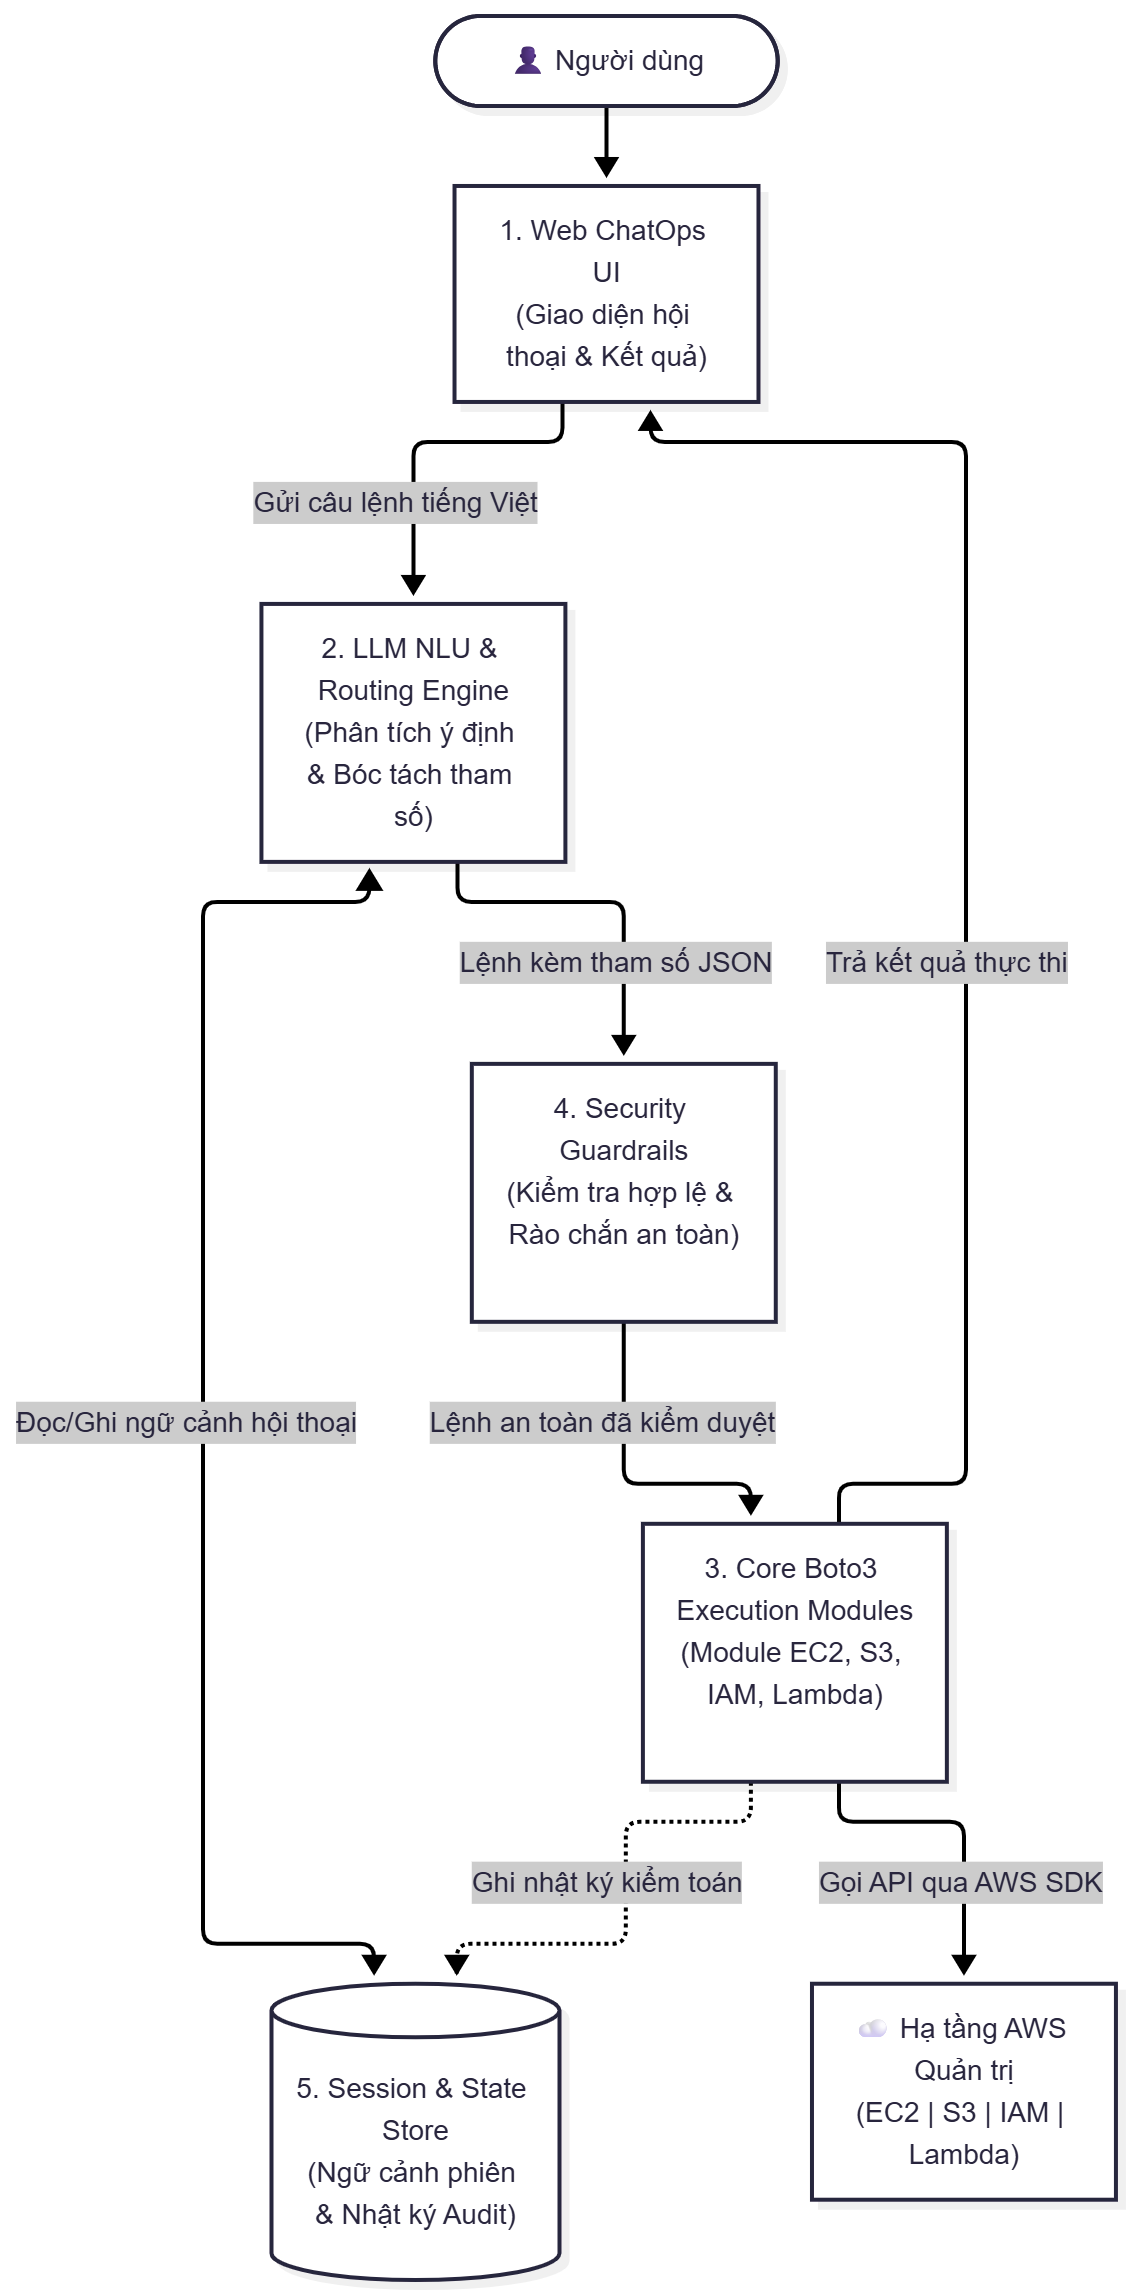
\includegraphics[width=0.68\textwidth,height=14.5cm,keepaspectratio]{kien_truc_tinh_nang.png}
}{
  \fbox{\parbox[c][5cm][c]{0.8\textwidth}{\centering Sơ đồ kiến trúc tính năng hệ thống SatiBot}}
}
\caption{Sơ đồ kiến trúc tính năng và luồng xử lý nghiệp vụ của SatiBot}
\label{fig:kientruc_tinhnang}
\end{figure}

Dựa trên sơ đồ kiến trúc tính năng (Hình~\ref{fig:kientruc_tinhnang}), các phân hệ chức năng cốt lõi của hệ thống được giải thích chi tiết như sau:

\begin{enumerate}
  \item \textbf{Phân hệ Giao diện trò chuyện và Tiếp nhận yêu cầu (Web ChatOps UI):}
  Đóng vai trò là điểm chạm duy nhất của người dùng với hệ thống. Giao diện cung cấp khung hội thoại thời gian thực, cho phép người dùng nhập câu lệnh yêu cầu bằng ngôn ngữ tự nhiên (ưu tiên tiếng Việt), hiển thị bảng dữ liệu định dạng chuẩn, cung cấp các liên kết bảo mật có thời hạn (Presigned URL / Function URL), các nút bấm xác nhận tác vụ nhạy cảm và biểu đồ/số liệu giám sát tài nguyên.

  \item \textbf{Phân hệ Xử lý Ngôn ngữ Tự nhiên \& Định tuyến Tác vụ (LLM NLU \& Routing Engine):}
  Tiếp nhận các chuỗi hội thoại tiếng Việt từ người dùng, làm giàu ngữ cảnh (context enrichment) bằng lịch sử trò chuyện gần nhất, sau đó gửi tới mô hình ngôn ngữ lớn (LLM). Tận dụng cơ chế \textit{Function Calling}, phân hệ này phân tích cú pháp, trích xuất chính xác tên hành động (action/tool) và các tham số kỹ thuật tương ứng dưới dạng dữ liệu JSON chuẩn hóa (ví dụ: tên máy ảo, loại instance, thời hạn presigned URL, dung lượng RAM...).

  \item \textbf{Phân hệ Thực thi AWS SDK \& Quản trị Dịch vụ (Core Boto3 Execution Modules):}
  Tập hợp các module chuyên trách độc lập viết bằng Python sử dụng thư viện AWS SDK (Boto3) để tương tác trực tiếp với các AWS API:
  \begin{itemize}
    \item \textit{Module EC2:} Quản lý máy chủ ảo, điều khiển chu kỳ hoạt động (Bật / Tắt / Khởi động lại / Xóa), kiểm tra vCPU quota và giám sát hiệu năng qua CloudWatch.
    \item \textit{Module S3:} Quản trị thùng chứa, rà soát và kích hoạt chặn truy cập công khai (Block Public Access), sinh liên kết tải có thời hạn (Presigned URL) và cấu hình quy tắc vòng đời lưu trữ (Lifecycle Rules).
    \item \textit{Module IAM:} Tra cứu vai trò và chính sách, sinh Role/Policy theo nguyên tắc đặc quyền tối thiểu (Least Privilege), cấp phát hoặc thu hồi quyền và xóa an toàn đối tượng IAM.
    \item \textit{Module Lambda:} Kiểm toán danh mục và cấu hình hàm, chạy thử nghiệm hàm trực tiếp qua Chat (Direct Invocation), tinh chỉnh cấu hình nóng (RAM \& Timeout), cấp phát nhanh Function URL và cơ chế dập cầu dao khẩn cấp (Kill-Switch).
  \end{itemize}

  \item \textbf{Phân hệ An toàn, Xác thực \& Rào chắn Bảo vệ (Security Guardrails):}
  Đóng vai trò là màng lọc bảo vệ hệ thống trước khi bất kỳ lệnh gọi API AWS nào được thực thi. Phân hệ này chịu trách nhiệm: (1) Kiểm tra tính hợp lệ và an toàn của tham số đầu vào; (2) Ngăn chặn các thao tác rủi ro cao (như mở cổng SSH 22 ra Internet 0.0.0.0/0, cấp quyền AdministratorAccess dư thừa); (3) Kích hoạt cơ chế xác nhận hai bước (two-step confirmation) đối với các thao tác phá hủy (xóa máy ảo, xóa bucket, thu hồi quyền); (4) Tính toán đối soát chi phí nhằm cảnh báo sớm việc vượt ngưỡng gói miễn phí (Free Tier).

  \item \textbf{Phân hệ Quản lý Phiên \& Lưu trữ Trạng thái (Session \& State Store):}
  Duy trì ngữ cảnh hội thoại đa lượt (multi-turn conversation) của từng người dùng, lưu trữ trạng thái các tác vụ đang chờ xác nhận (pending confirmation state) và ghi lại toàn bộ nhật ký tương tác phục vụ mục đích kiểm toán (audit log) và giám sát hệ thống.
\end{enumerate}

\subsection{Kiến trúc triển khai của hệ thống}

Kiến trúc triển khai của SatiBot được xây dựng hoàn toàn trên nền tảng Serverless của AWS nhằm đạt được tính sẵn sàng cao (High Availability), khả năng tự động mở rộng theo tải (Auto-scaling) và tối ưu hóa chi phí vận hành (chỉ trả phí cho thời gian thực thi thực tế).

Bảng~\ref{tab:kientruc} tổng hợp chi tiết các thành phần và dịch vụ được đề xuất sử dụng trong kiến trúc triển khai của hệ thống.

\begin{table}[htbp]
\centering
\caption{Các thành phần và dịch vụ đề xuất trong kiến trúc hệ thống}
\label{tab:kientruc}
\bangfont
\begin{tabularx}{\linewidth}{@{}p{4.8cm}Y@{}}
\toprule
\textbf{Thành phần / Dịch vụ} & \textbf{Vai trò dự kiến}\\
\midrule
React & Xây dựng giao diện ứng dụng web (Frontend).\\
Amazon S3 \& Amazon CloudFront & Lưu trữ static file và phân phối giao diện web đến người dùng với tốc độ cao, hỗ trợ bảo mật HTTPS.\\
Amazon Cognito & Quản lý xác thực, đăng ký và đăng nhập người dùng ứng dụng web, cấp phát JWT token.\\
Amazon API Gateway & Tiếp nhận và định tuyến các yêu cầu HTTP/HTTPS từ Frontend đến Backend, tích hợp xác thực token.\\
AWS Lambda & Chạy phần xử lý trung tâm (Backend serverless) của ứng dụng, tự động mở rộng quy mô.\\
Python / Boto3 & Ngôn ngữ và thư viện AWS SDK được triển khai trong Lambda Backend để gọi các AWS API tương ứng.\\
LLM & Mô hình ngôn ngữ lớn phân tích ngữ cảnh yêu cầu của người dùng và hỗ trợ cơ chế \textit{function calling} (chưa chốt nhà cung cấp hoặc mô hình cụ thể).\\
Amazon DynamoDB & Cơ sở dữ liệu NoSQL lưu trữ lịch sử hội thoại, các tham số và trạng thái tác vụ.\\
Amazon CloudWatch & Ghi log hệ thống và theo dõi hoạt động vận hành của các dịch vụ backend.\\
AWS IAM & Thiết lập, cấp phát và kiểm soát quyền truy cập giữa các thành phần trong hệ thống.\\
\bottomrule
\end{tabularx}
\end{table}

Kiến trúc triển khai của hệ thống được thiết kế theo mô hình phân tầng từ mức tổng quan đến các phân hệ chi tiết, làm rõ luồng dữ liệu và giao diện tương tác giữa các dịch vụ trên nền tảng AWS.

\subsubsection{Sơ đồ kiến trúc triển khai tổng thể (Mức cao)}

Sơ đồ Hình~\ref{fig:trien_khai1} mô tả bức tranh toàn cảnh kết nối giữa 04 khối thành phần chính của hệ thống SatiBot.

\begin{figure}[H]
\centering
\IfFileExists{trien_khai1.png}{
  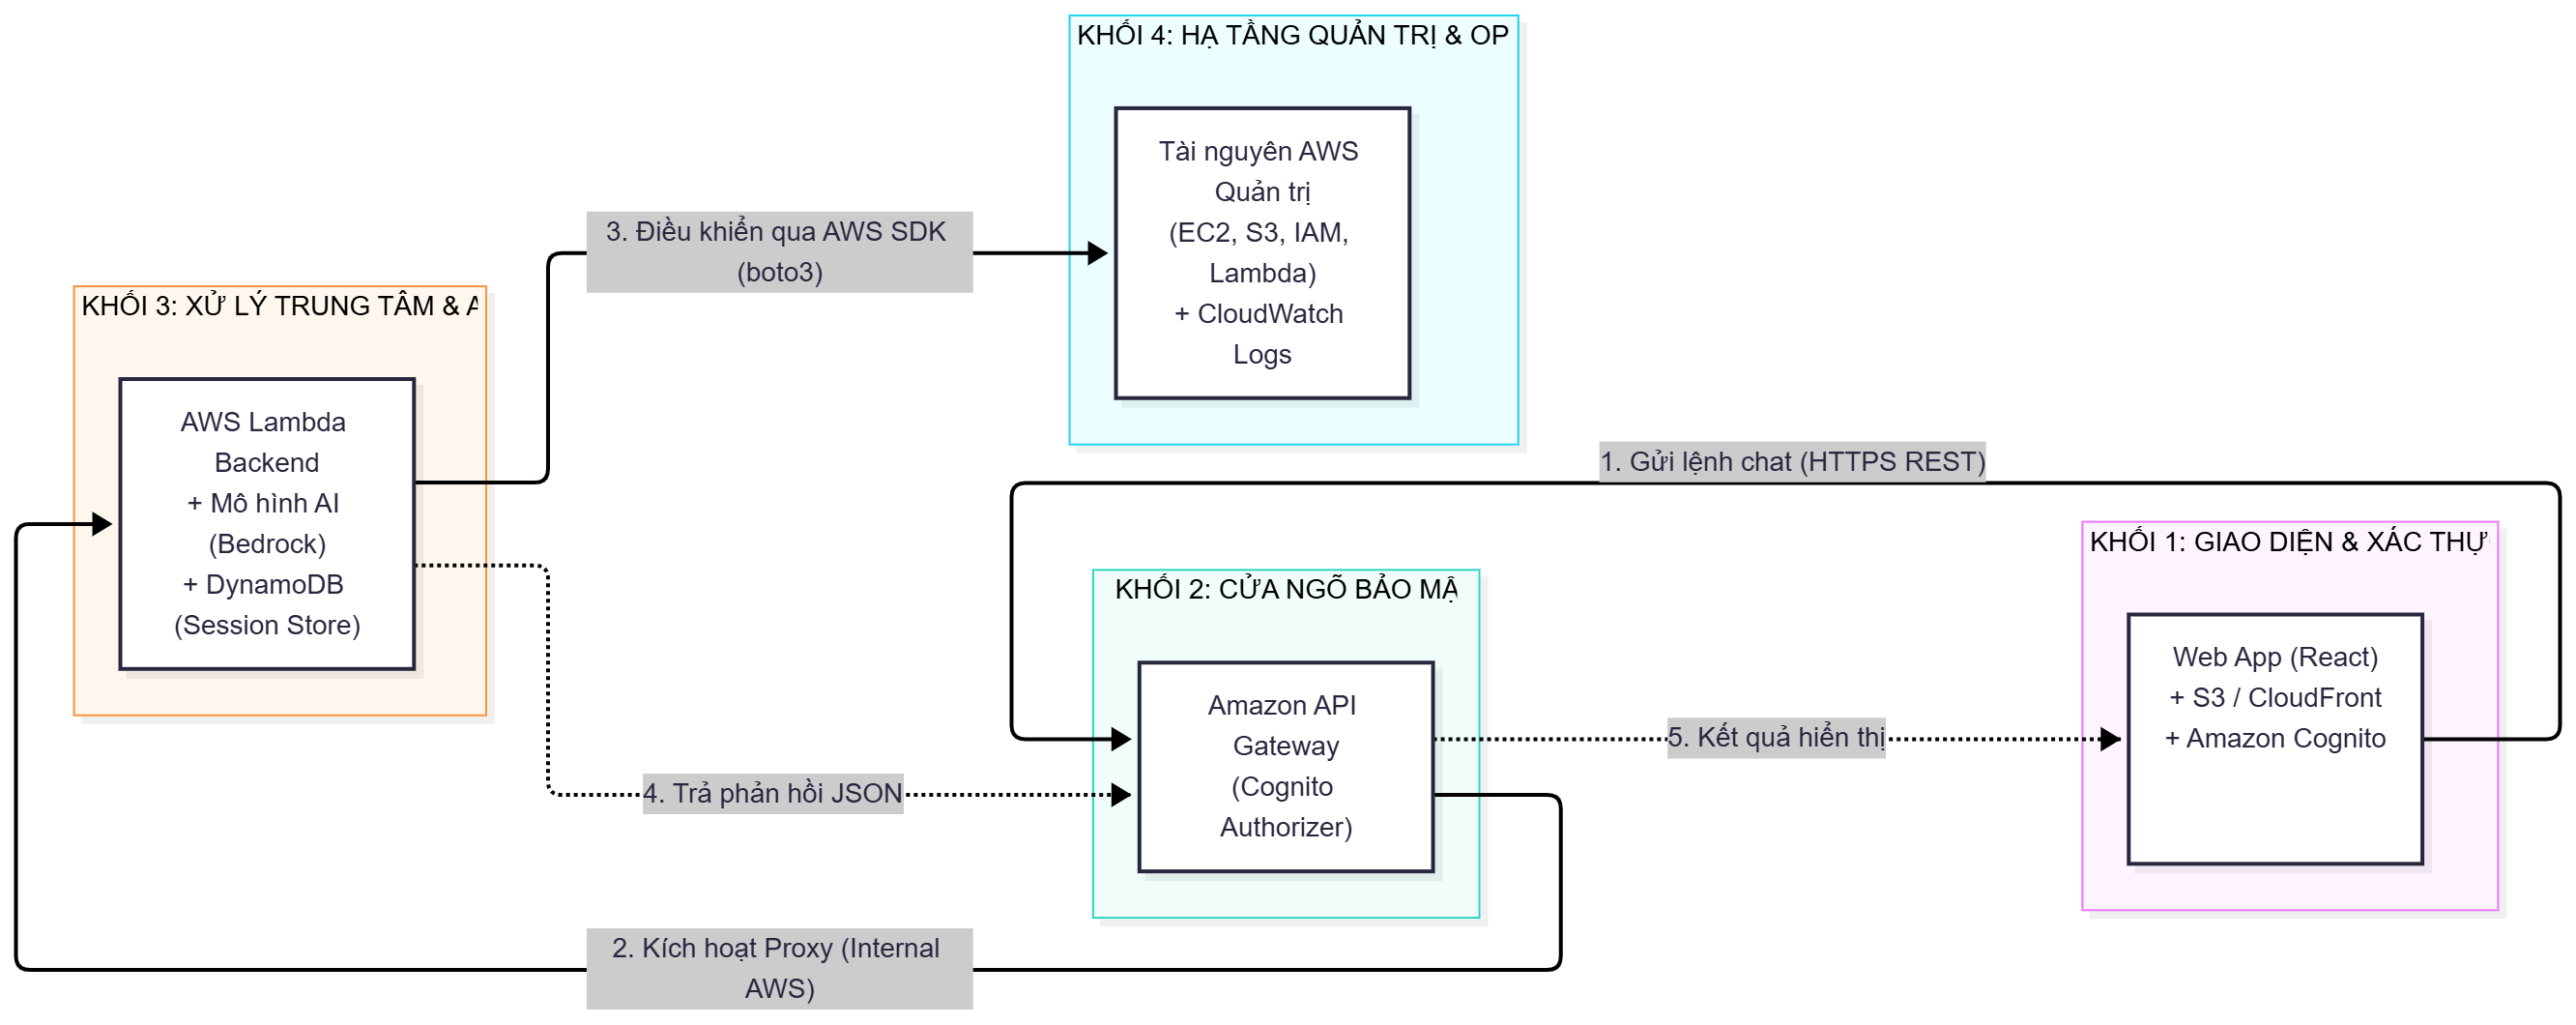
\includegraphics[width=0.95\textwidth]{trien_khai1.png}
}{
  \fbox{\parbox[c][5cm][c]{0.8\textwidth}{\centering Sơ đồ kiến trúc triển khai tổng quan}}
}
\caption{Sơ đồ kiến trúc triển khai tổng quan hệ thống SatiBot (Mức cao)}
\label{fig:trien_khai1}
\end{figure}

Kiến trúc tổng thể hoạt động qua 04 khối chức năng:
\begin{itemize}
  \item \textbf{Khối 1 (Giao diện \& Xác thực):} Người dùng tương tác với Web App (React) được phân phối qua S3/CloudFront và xác thực qua Amazon Cognito.
  \item \textbf{Khối 2 (Cửa ngõ bảo mật):} Amazon API Gateway tiếp nhận lệnh chat từ người dùng qua giao thức HTTPS REST và kiểm tra tính hợp lệ của JWT token thông qua Cognito Authorizer.
  \item \textbf{Khối 3 (Xử lý trung tâm \& AI):} AWS Lambda tiếp nhận request qua cơ chế kích hoạt Proxy nội bộ của AWS, phối hợp cùng mô hình AI (Bedrock) và Amazon DynamoDB để phân tích ngữ cảnh, sinh lệnh kỹ thuật và trả phản hồi JSON.
  \item \textbf{Khối 4 (Hạ tầng quản trị \& Ops):} Lambda điều khiển trực tiếp 04 dịch vụ AWS mục tiêu (EC2, S3, IAM, Lambda) thông qua AWS SDK (Boto3) và tự động đẩy nhật ký hoạt động sang Amazon CloudWatch Logs.
\end{itemize}

\subsubsection{Chi tiết Phân hệ Giao diện, Xác thực và Cửa ngõ API (Khối 1 \& 2)}

Sơ đồ Hình~\ref{fig:trien_khai2} làm rõ chi tiết quy trình người dùng truy cập, đăng nhập và gửi lệnh vào cửa ngõ hệ thống.

\begin{figure}[H]
\centering
\IfFileExists{trien_khai2.png}{
  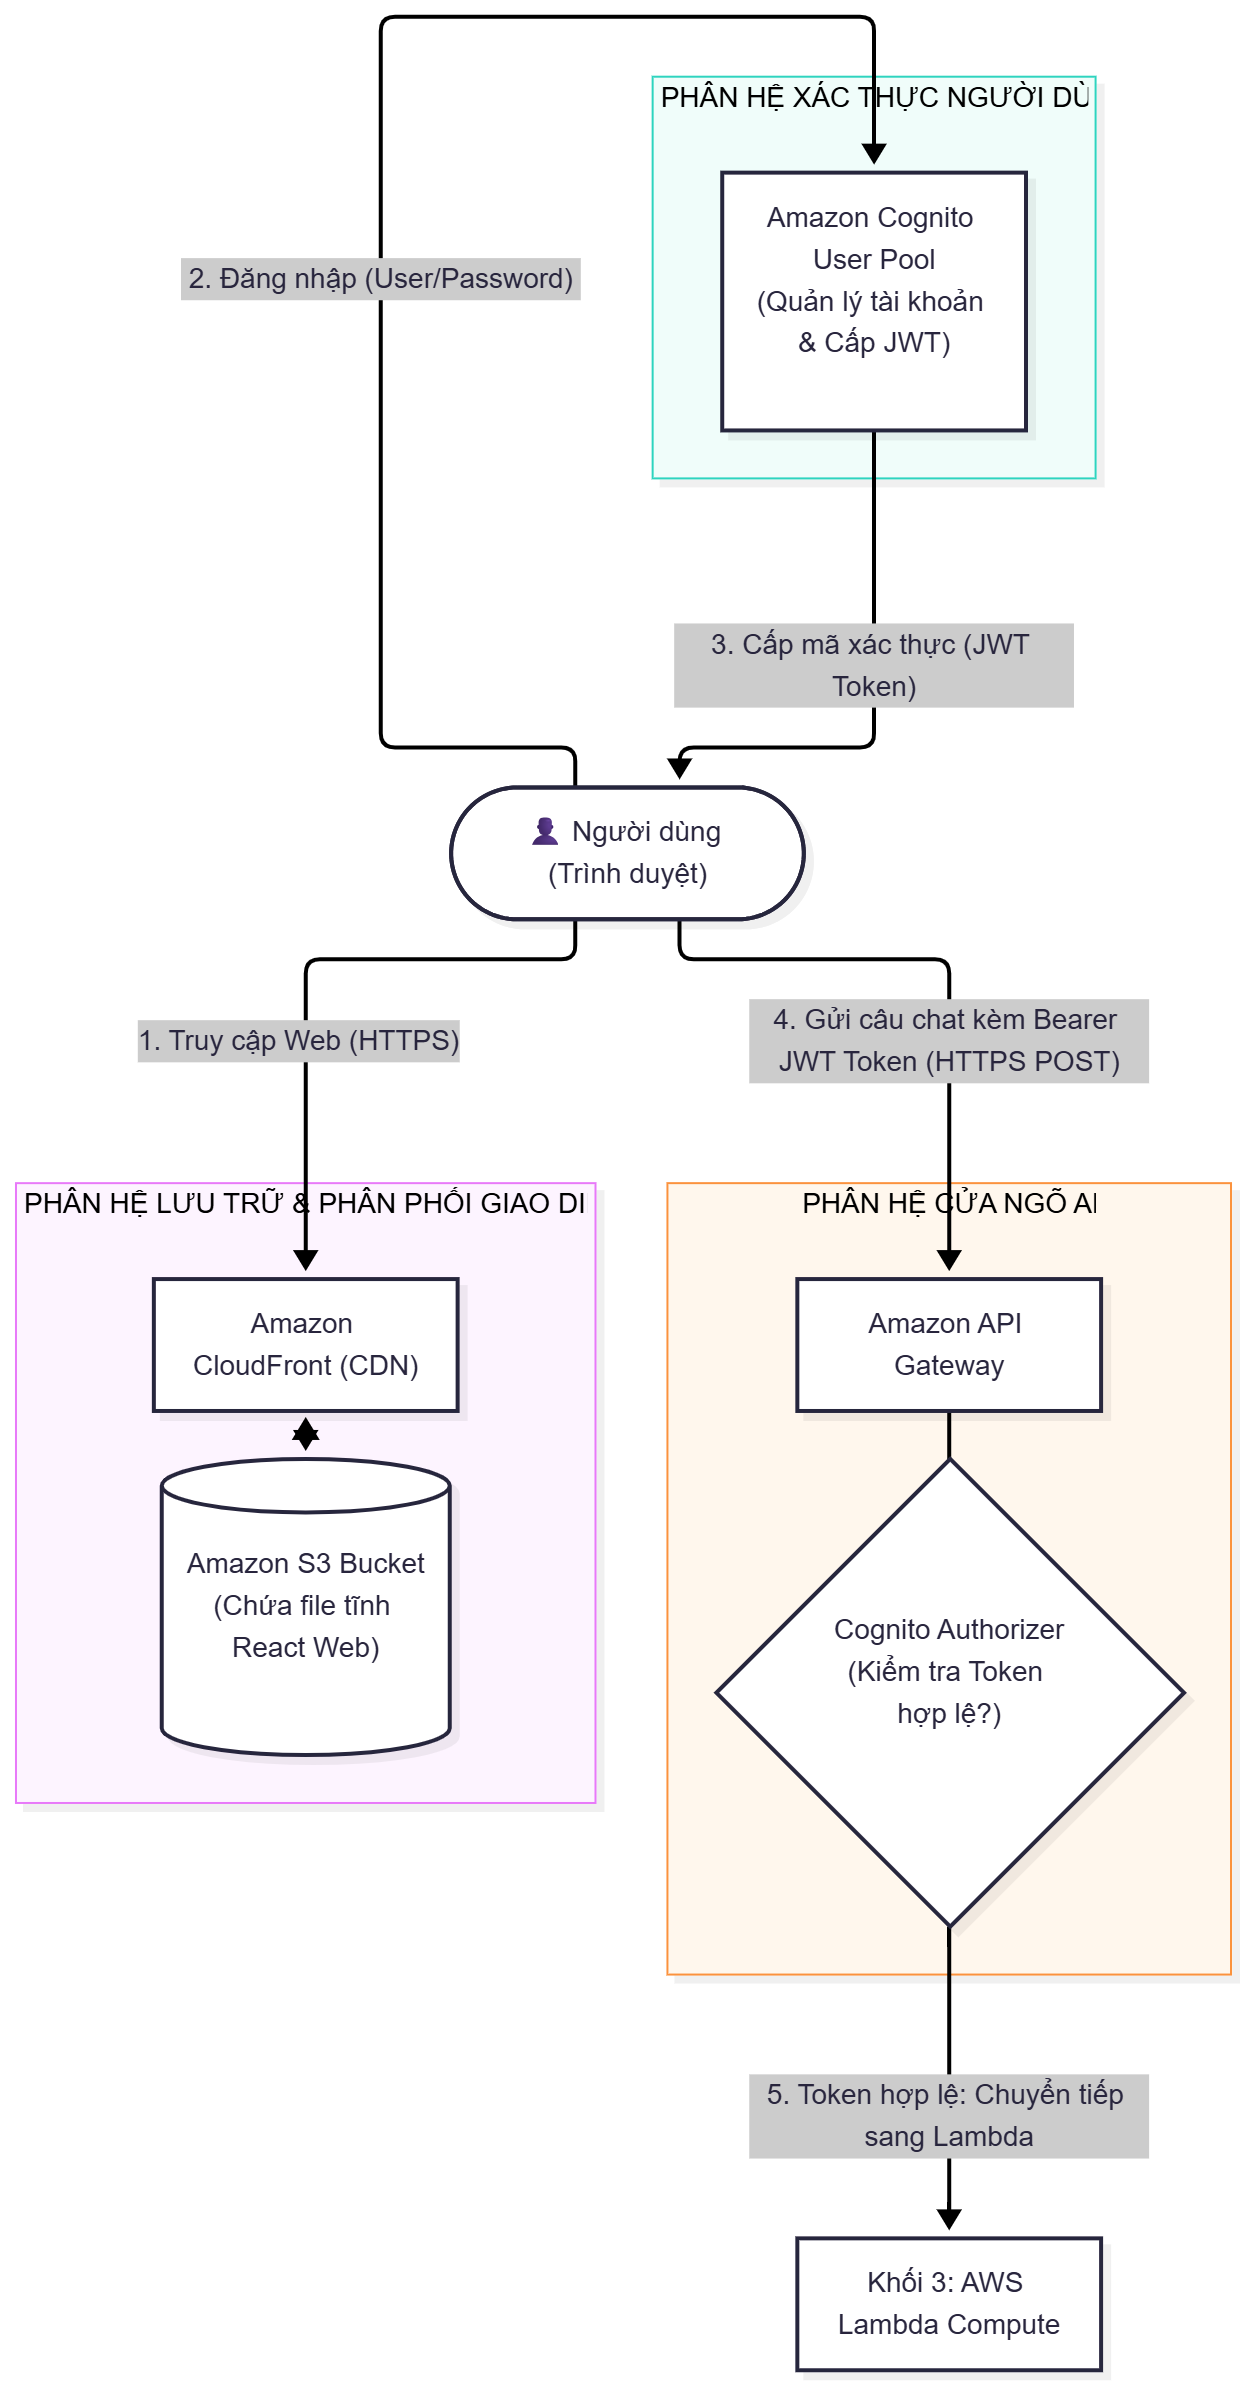
\includegraphics[height=11.5cm,keepaspectratio]{trien_khai2.png}
}{
  \fbox{\parbox[c][5cm][c]{0.8\textwidth}{\centering Chi tiết phân hệ Giao diện, Xác thực và Cửa ngõ API}}
}
\caption{Sơ đồ chi tiết phân hệ Giao diện, Xác thực và Cửa ngõ API}
\label{fig:trien_khai2}
\end{figure}

Quy trình tương tác diễn ra tuần tự qua các bước:
\begin{enumerate}
  \item \textbf{Truy cập Web:} Người dùng truy cập website qua giao thức HTTPS; Amazon CloudFront tối ưu hóa tốc độ tải và lấy các tệp tĩnh (HTML, CSS, JS) từ Amazon S3 Bucket riêng tư.
  \item \textbf{Xác thực người dùng:} Người dùng nhập tài khoản (User/Password); Amazon Cognito User Pool thẩm định thông tin và cấp mã xác thực JWT Token (gồm ID Token và Access Token) về cho trình duyệt.
  \item \textbf{Gửi lệnh chat:} Người dùng nhập câu lệnh tiếng Việt; trình duyệt gửi HTTPS POST request đính kèm Bearer JWT Token vào tiêu đề (Authorization header) tới Amazon API Gateway.
  \item \textbf{Kiểm tra bảo mật tại cổng:} Cognito Authorizer tích hợp tại API Gateway giải mã và kiểm tra chữ ký số của token. Nếu token không hợp lệ, yêu cầu bị chặn ngay lập tức (trả về mã 401). Nếu hợp lệ, API Gateway kích hoạt chuyển tiếp yêu cầu sang Khối 3 (AWS Lambda Compute).
\end{enumerate}

\subsubsection{Chi tiết Phân hệ Xử lý Trung tâm và Trí tuệ Nhân tạo (Khối 3)}

Sơ đồ Hình~\ref{fig:trien_khai3} mô tả luồng điều phối thông minh, làm giàu ngữ cảnh và cơ chế rào chắn an toàn bên trong hàm AWS Lambda.

\begin{figure}[H]
\centering
\IfFileExists{trien_khai3.png}{
  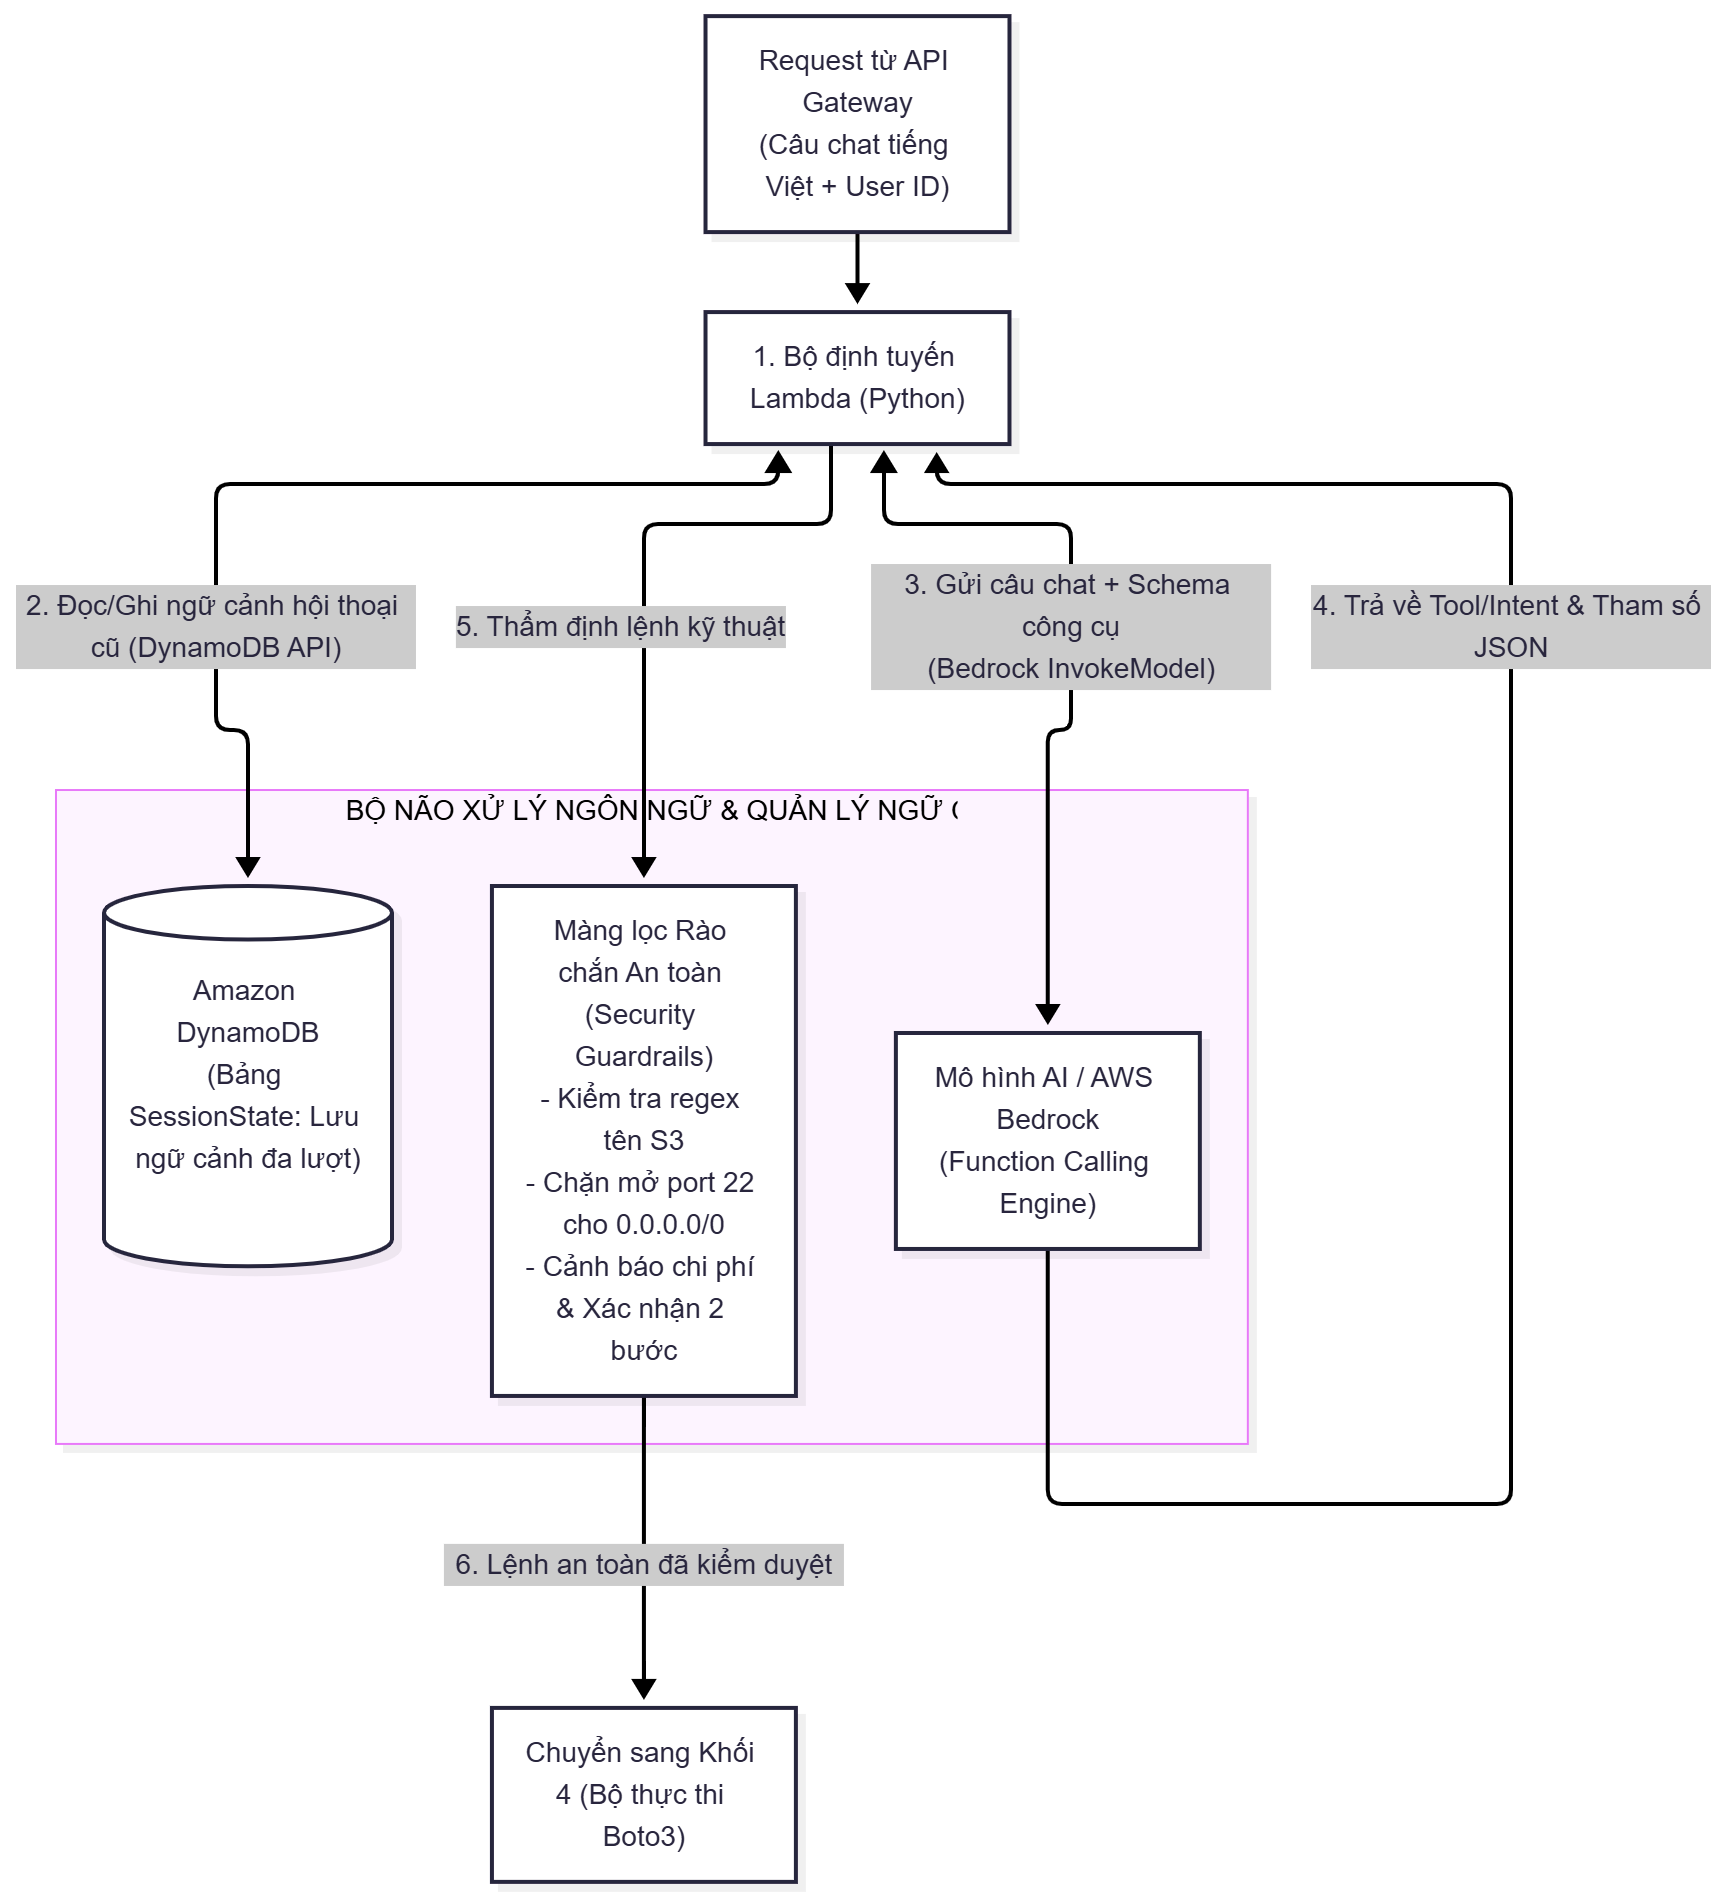
\includegraphics[height=12cm,keepaspectratio]{trien_khai3.png}
}{
  \fbox{\parbox[c][5cm][c]{0.8\textwidth}{\centering Chi tiết phân hệ Xử lý Trung tâm và Trí tuệ Nhân tạo}}
}
\caption{Sơ đồ chi tiết phân hệ Xử lý Trung tâm và Trí tuệ Nhân tạo}
\label{fig:trien_khai3}
\end{figure}

Các bước xử lý logic trung tâm bao gồm:
\begin{enumerate}
  \item \textbf{Tiếp nhận yêu cầu:} Bộ định tuyến Lambda (Python) tiếp nhận payload từ API Gateway gồm câu chat tiếng Việt và định danh người dùng (User ID).
  \item \textbf{Làm giàu ngữ cảnh:} Lambda gọi API DynamoDB để đọc/ghi lịch sử hội thoại gần nhất từ bảng \texttt{SessionState}, đảm bảo hệ thống hiểu được ngữ cảnh hội thoại đa lượt.
  \item \textbf{Suy luận và trích xuất tham số (AI Bedrock):} Lambda gửi câu chat cùng bộ đặc tả công cụ (Tool Schema) tới mô hình AI trên AWS Bedrock qua API \texttt{InvokeModel}. Tận dụng cơ chế \textit{Function Calling}, mô hình AI trả về cấu trúc JSON chứa tên công cụ (Tool/Intent) và các tham số kỹ thuật bóc tách được.
  \item \textbf{Kiểm duyệt qua Rào chắn An toàn (Security Guardrails):} Trước khi thực thi, câu lệnh kỹ thuật bắt buộc phải đi qua màng lọc kiểm duyệt an toàn: (1) Kiểm tra biểu thức chính quy (regex) đặt tên bucket S3 hợp lệ; (2) Chặn tuyệt đối hành vi mở cổng SSH 22 ra dải IP toàn cầu 0.0.0.0/0; (3) Tính toán chi phí dự kiến và kích hoạt quy trình xác nhận hai bước đối với các lệnh nhạy cảm (xóa tài nguyên, cấp quyền cao). Khi đáp ứng toàn bộ tiêu chí an toàn, lệnh mới được bàn giao sang Khối 4 để thực thi.
\end{enumerate}

\subsubsection{Chi tiết Phân hệ Điều phối Boto3, Quản trị Tài nguyên và Giám sát (Khối 4)}

Sơ đồ Hình~\ref{fig:trien_khai4} thể hiện cấu trúc các module thực thi mã nguồn Boto3, sự tương tác với các tài nguyên AWS đích và cơ chế lưu trữ vết giám sát.

\begin{figure}[H]
\centering
\IfFileExists{trien_khai4.png}{
  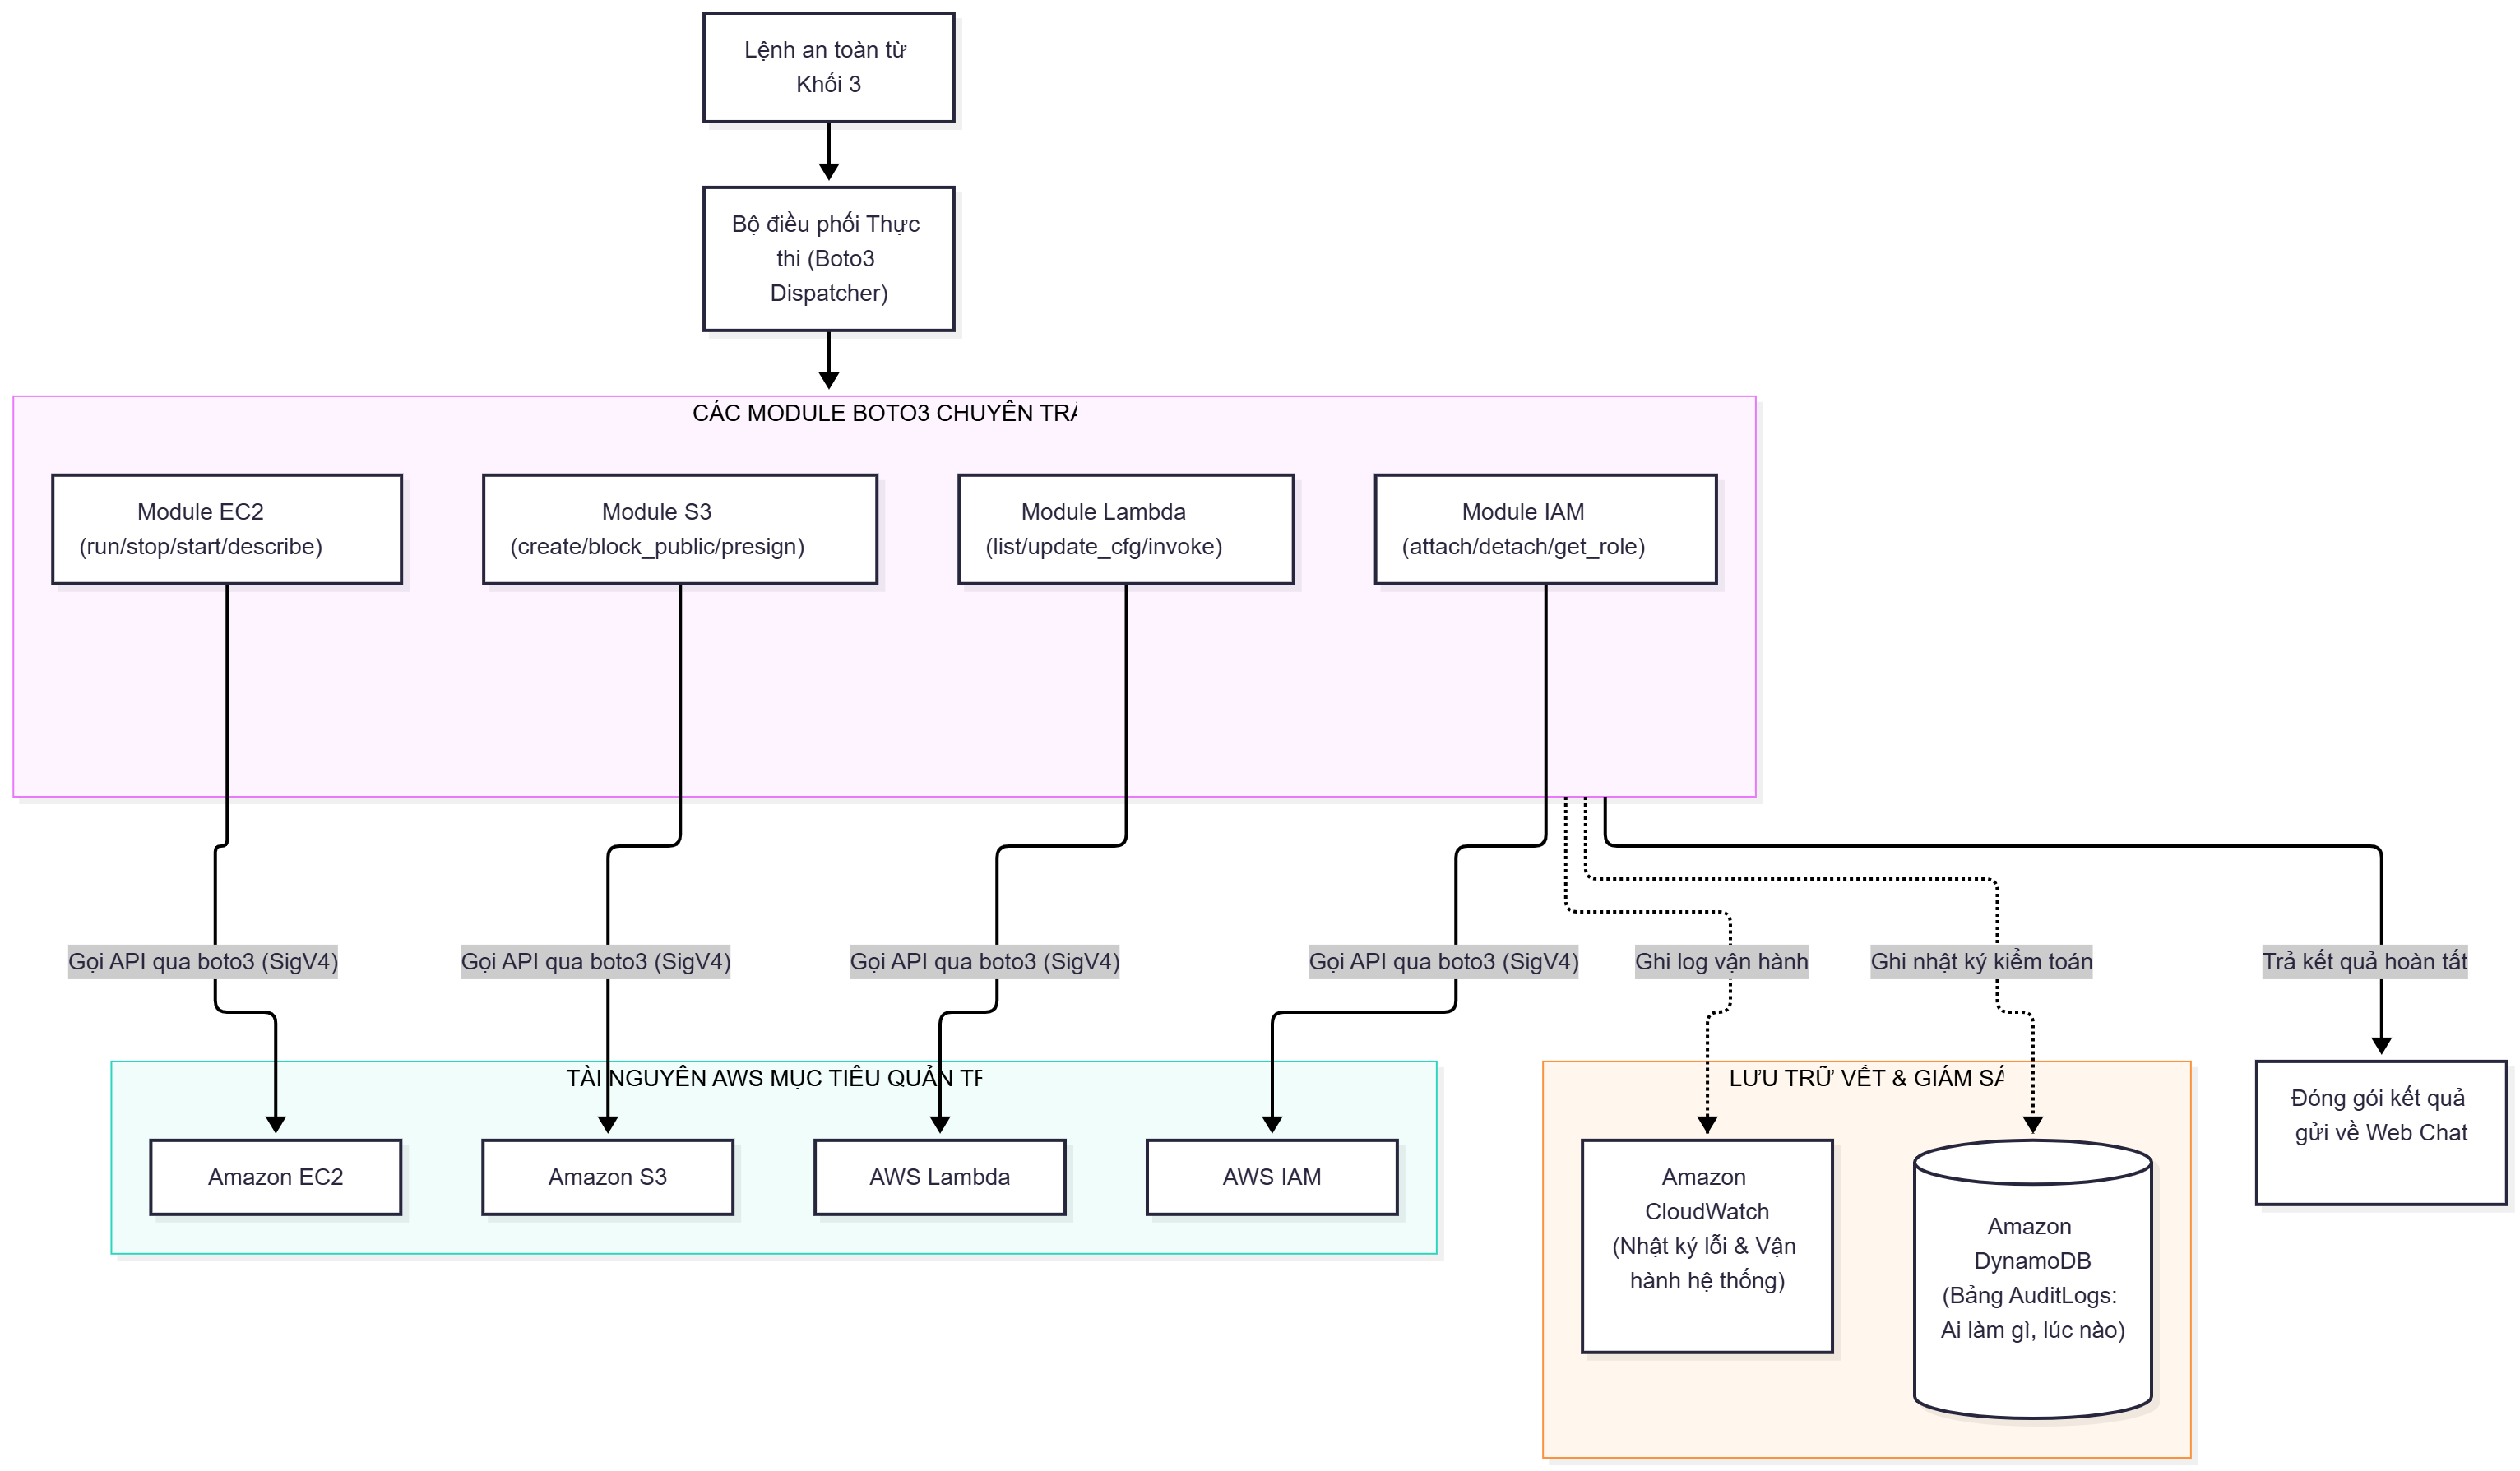
\includegraphics[width=0.95\textwidth]{trien_khai4.png}
}{
  \fbox{\parbox[c][5cm][c]{0.8\textwidth}{\centering Chi tiết phân hệ Điều phối Boto3, Quản trị Tài nguyên và Giám sát}}
}
\caption{Sơ đồ chi tiết phân hệ Điều phối Boto3, Quản trị Tài nguyên và Giám sát}
\label{fig:trien_khai4}
\end{figure}

Cơ chế vận hành của phân hệ quản trị và giám sát:
\begin{enumerate}
  \item \textbf{Điều phối thực thi (Boto3 Dispatcher):} Nhận lệnh an toàn từ Khối 3 và chuyển giao chính xác cho module Boto3 chuyên trách:
  \begin{itemize}
    \item \textit{Module EC2:} Quản lý máy ảo (\texttt{run\_instances}, \texttt{stop}, \texttt{start}, \texttt{describe}).
    \item \textit{Module S3:} Quản lý thùng chứa (\texttt{create\_bucket}, \texttt{block\_public}, \texttt{presign}).
    \item \textit{Module Lambda:} Quản lý hàm (\texttt{list\_functions}, cấu hình \texttt{config}, gọi \texttt{invoke}).
    \item \textit{Module IAM:} Quản lý quyền (\texttt{attach\_role\_policy}, \texttt{detach}, \texttt{get\_role}).
  \end{itemize}
  \item \textbf{Xác thực và ủy quyền:} Toàn bộ các cuộc gọi API tới 04 dịch vụ AWS đích đều sử dụng chữ ký điện tử AWS SigV4 được cấp phát động thông qua IAM Execution Role của hàm Lambda, tuân thủ nguyên tắc đặc quyền tối thiểu (Least Privilege).
  \item \textbf{Lưu vết kiểm toán và giám sát:}
  \begin{itemize}
    \item Hệ thống tự động đẩy nhật ký vận hành và thông báo lỗi sang Amazon CloudWatch Logs để phục vụ giám sát và gỡ lỗi.
    \item Ghi nhận vết kiểm toán chi tiết (người dùng nào thực hiện, thao tác gì, tác động lên tài nguyên nào, vào thời điểm nào) vào bảng AuditLogs trên Amazon DynamoDB nhằm đảm bảo tính minh bạch và bảo mật.
  \end{itemize}
  \item \textbf{Đóng gói và phản hồi:} Sau khi hoàn tất thao tác trên AWS, kết quả thực thi được định dạng chuẩn hóa và trả ngược về Web Chat dưới dạng bảng biểu hoặc thông báo trực quan cho người dùng.
\end{enumerate}

\clearpage

\section{KẾ HOẠCH TRIỂN KHAI VÀ ƯỚC TÍNH NỖ LỰC}


\end{document}
